\documentclass[a4paper, 12pt]{article} % Artikel-Klasse

%---------------------------------------------------------
% Encoding, language, quotes
%---------------------------------------------------------
\usepackage[utf8]{inputenc}
\usepackage[ngerman]{babel}       % Deutsche Sprache und Silbentrennung
\usepackage{csquotes}             % Für korrekte Anführungszeichen
\usepackage{listings}
\usepackage{xcolor}

%---------------------------------------------------------
% Graphics & PDF
%---------------------------------------------------------
\usepackage{graphicx}
\usepackage{pdfpages}             % Einbinden von PDF-Seiten
\usepackage{caption}              % Verbesserte Bildunterschriften
\usepackage{subcaption}
\usepackage{comment}


% Customize settings
% Customize settings for a more compact style
\lstset{
    language=Java,                 % Specify Java language for syntax highlighting
    basicstyle=\ttfamily\small,    % Use smaller monospaced font for code
    keywordstyle=\color{blue},     % Style for keywords
    commentstyle=\color{gray},     % Style for comments
    stringstyle=\color{red},       % Style for strings
    numbers=none,                  % No line numbers
    breaklines=true,               % Break long lines
    frame=none,                    % No frame around the code
    xleftmargin=0pt,               % Remove left margin
    xrightmargin=0pt,              % Remove right margin
    aboveskip=5pt,                 % Reduce space above the code block
    belowskip=5pt                  % Reduce space below the code block
}

%---------------------------------------------------------
% Math, units, spacing, etc.
%---------------------------------------------------------
\usepackage{siunitx}
\usepackage{setspace}
\usepackage{textgreek}

% Add float package for "H" float option
\usepackage{float}

%---------------------------------------------------------
% Other packages
%---------------------------------------------------------
\usepackage{ifthen}
\usepackage{acronym}
\PassOptionsToPackage{hyphens}{url} % URLs in Hyperlinks umbrechen
\usepackage[breaklinks=true]{hyperref} 
\usepackage{array}                % Bessere Tabellenformatierung
\usepackage{enumitem}             % Kontrolle über Listen-Layouts
\usepackage{nomencl}
\usepackage{scrlayer-scrpage}     % Header und Footer

% Adjust header and footer heights
\setlength{\headheight}{14.5pt}
\setlength{\footheight}{34.16666pt}

%---------------------------------------------------------
% Bibliography (biblatex mit Biber)
%---------------------------------------------------------
\usepackage[backend=biber, style=numeric]{biblatex}  

\addbibresource{literatur.bib}  

%---------------------------------------------------------
% Platzhalter
%---------------------------------------------------------
\newcommand{\titel}{Umbau und Inbetriebnahme eines Konzeptfahrzeugs zur Erprobung eines neuen Fahrantriebs}
\newcommand{\untertitel}{}
\newcommand{\arbeit}{T3000 Hausarbeit}
\newcommand{\studiengang}{Elektrotechnik}
\newcommand{\studienrichtung}{Fahrzeugelektronik}
\newcommand{\autor}{Luka Tadic}
\newcommand{\abgabe}{14.04.2025}
\newcommand{\bearbeitungszeitraum}{19.01.2025 – 14.04.2025}
\newcommand{\matrikelnr}{5726700}
\newcommand{\kurs}{TFE22–1} % en-dash used here
\newcommand{\firma}{Kramer Werke GmbH}
\newcommand{\betreuerfirma}{Dipl. Ing. Christian Borgmann}
\newcommand{\gutachterdhbw}{Prof.\ Dr.\ Ing. Konrad Reif}
\newcommand{\jahr}{2025}

%---------------------------------------------------------
% Header und Footer mit Linien
%---------------------------------------------------------
\clearpairofpagestyles{}

% Header with consistent logo placement for two logos and line position
\ohead{%
    \parbox{\textwidth}{% Create a flexible container for both images
        \raisebox{1.5cm}[0pt][0pt]{% Raise the Kramer logo
            
\includegraphics[width=3cm]{images/kramer.png}%
        }%
        \hfill % Horizontal space between the two logos
        \raisebox{1.5cm}[0pt][0pt]{% Raise the DHBW logo
            
\includegraphics[width=3cm]{images/DHBW_d_R_FN_46mm_4c}%
        }%
    }%
    \\[-1.5cm] % Move the header line down
    \rule{\textwidth}{0.4pt} % Horizontal rule for the header line
}


% Footer with consistent alignment and contents below the line
\setkomafont{pagefoot}{\normalfont} % Ensure consistent font style
\cfoot{%
    \rule{\textwidth}{0.4pt}\\ % Horizontal rule
    \vspace{0.3em} % Small vertical space
    \begin{tabular}{@{}p{0.33\textwidth}p{0.33\textwidth}p{0.33\textwidth}@{}}
        \arbeit~& \centering \autor~& \raggedleft~\thepage%
    \end{tabular}
}


\pagestyle{scrheadings}        % Stil aktivieren

%---------------------------------------------------------
% Dokumentbeginn
%---------------------------------------------------------
\begin{document}
\sloppy

%---------------------------------------------------------
% Titelseite
%---------------------------------------------------------
\thispagestyle{empty}  % Kein Header oder Footer auf der Titelseite
\hypersetup{pageanchor=false}

\begin{titlepage}
\enlargethispage{4.0cm}
\sffamily  % Serifenlose Schrift für die Titelseite

% Create a container for both logos at the top
\parbox{0.5\linewidth}{%
    \begin{flushleft}
        
\includegraphics[width=0.4\linewidth]{images/kramer.png}\\[5ex] % Kramer logo on the left
    \end{flushleft}
}
\parbox{0.5\linewidth}{%
    \begin{flushright}
        
\includegraphics[width=0.4\linewidth]{images/DHBW_d_R_FN_46mm_4c}\\[5ex] % DHBW logo on the right
    \end{flushright}
}

% Title and information in the center
\begin{center}

{\fontsize{20.74pt}{24pt}\selectfont
\textbf{\titel}\\[1.5ex]}

{\fontsize{17pt}{20pt}\selectfont
\textbf{\arbeit}\\[2ex]}

{\fontsize{14pt}{17pt}\selectfont
Studiengang \studiengang\\[2ex]}

{\fontsize{12pt}{14pt}\selectfont
Studienrichtung \studienrichtung\\[1ex]
Duale Hochschule Baden-Württemberg Ravensburg, Campus Friedrichshafen\\[5ex]
von\\[1ex]
\autor\\[15ex]}

\end{center}

% Footer-like table with additional information
\begin{center}
{\fontsize{12pt}{14pt}\selectfont
\begin{tabular}{ll}
Abgabedatum:                    & \quad \abgabe\\  
Bearbeitungszeitraum:           & \quad \bearbeitungszeitraum\\  
Matrikelnummer:                 & \quad \matrikelnr\\ 
Kurs:                           & \quad \kurs\\ 
Dualer Partner:                 & \quad \firma\\ % entfällt bei Studienarbeit
Betreuerin / Betreuer:          & \quad \betreuerfirma\\  
Gutachterin / Gutachter:        & \quad \gutachterdhbw\\ [2ex]
\end{tabular}
}
\end{center}

\end{titlepage}

\clearpage

\pagestyle{scrheadings}  % Header und Footer nach Titelseite aktivieren
\hypersetup{pageanchor=true}

%---------------------------------------------------------
% Erklärung
%---------------------------------------------------------

\pagenumbering{Roman}

\section*{Erklärung}

Ich versichere hiermit, dass ich meine \arbeit\ mit dem Thema:

\begin{quote}
    \textit{\titel}
\end{quote}

selbstständig verfasst und keine anderen als die angegebenen Quellen und Hilfsmittel benutzt habe.  
Ich versichere zudem, dass die eingereichte elektronische Fassung mit der gedruckten Fassung übereinstimmt.\\[6ex]

Friedrichshafen, den \today \\[1ex]
\rule[-0.2cm]{5cm}{0.5pt} \\  
\autor\\[10ex]

\rmfamily

\clearpage

\section*{Kurzfassung}
\begin{spacing}{1.8}  % Adjust line spacing
    \fontsize{14pt}{14pt}\selectfont  % Font size and line spacing
    Im Rahmen dieses Projekts wird ein \acf{PoC}-Umbau an einem Kramer 415–38 Fahrzeug durchgeführt, 
    um die Praxistauglichkeit eines neuen Fahrantriebskonzepts zu überprüfen. Ziel ist es, die Leistung, 
    Dynamik und Reststeigfähigkeit des Fahrzeugs zu verbessern sowie Geräusch- und Kraftstoffverbrauch zu reduzieren.

    Der Umbau umfasst die Integration neuer Komponenten, darunter der Danfoss \ac{BPC}-Fahrantrieb, 
    eine Servobremse mit Hill-Hold-Funktion, das Rafi Gen2 Display sowie der Einbau der neuen Keypads 
    mit unterschiedlichen Fahrmodi Optionen. Die Umsetzung erfolgt in Zusammenarbeit mit Claus Vogt (mechanischer Umbau) und 
    Daniel Sessler (Softwareintegration). Nach dem Einbau wird das Fahrzeug getestet, um zu evaluieren, ob die gewünschten Effekte erreicht wurden.
    
    Das Projekt soll zeigen, ob sich das neue Fahrantriebskonzept erfolgreich in die T07/T08-Fahrzeugreihe integrieren lässt und somit die Wettbewerbsfähigkeit der Kramer Telelader steigert.
\end{spacing}

\clearpage
%---------------------------------------------------------
% Abstract
%---------------------------------------------------------
\section*{Abstract}
\begin{spacing}{1.8}  % Adjust line spacing
    \fontsize{14pt}{14pt}\selectfont  % Font size and line spacing
    As part of this project, a \acf{PoC} conversion is being carried out on a Kramer 415–38 
    vehicle to evaluate the feasibility of a new drive system concept. The goal is to 
    improve the vehicle's performance, dynamics, and gradeability while reducing noise and fuel consumption.

    The conversion includes integrating new components such as the Danfoss \ac{BPC} drive system, 
    a servo brake with a hill-hold function, the Rafi Gen2 display, and the installation of new 
    keypads with different drive mode options. The implementation is carried out in collaboration with Claus Vogt 
    (mechanical conversion) and Daniel Sessler (software integration). After installation, the vehicle 
    will be tested to assess whether the desired effects have been achieved.
    
    The project aims to determine whether the new drive system concept can be successfully 
    integrated into the T07/T08 vehicle series, thereby enhancing the competitiveness of Kramer telehandlers.

\end{spacing}
\clearpage

% List of figures
\listoffigures

\clearpage

\section*{Abkürzungsverzeichnis}
\begin{spacing}{1.8}  % Adjust line spacing
    \fontsize{14pt}{14pt}\selectfont  % Font size and line spacing

\begin{acronym}
    \acro{PoC}{Proof of Concept}
    \acro{BPC}{Best Point Control}
    \acro{SAP}{Systemanalyse Programmentwicklung}
\end{acronym}

\end{spacing}

\clearpage


%---------------------------------------------------------
% Inhaltsverzeichnis
%---------------------------------------------------------
\tableofcontents

\clearpage
\pagenumbering{arabic}


\section{Einleitung und Motivation}
\begin{spacing}{1.5}  % Adjust line spacing
\fontsize{14pt}{14pt}\selectfont  % Font size and line spacing
Im Rahmen dieses \acf{PoC}-Umbaus wird untersucht, ob das 
geplante Fahrantriebskonzept für die T07/T08-Modelle der Kramer-Telelader 
die gewünschten Verbesserungen hinsichtlich Leistung, Dynamik und 
Reststeigfähigkeit erzielt. Ziel des Projekts ist es, die Wettbewerbsfähigkeit
 der Fahrzeuge weiter zu steigern, indem innovative Technologien und 
 Optimierungsmaßnahmen implementiert werden.

Der Ausgangspunkt für diese Entwicklung waren die Ergebnisse des
 „Voice of Sales/Voice of Engineering“-Events im Juli 2021, bei dem 
 spezifische Anforderungen an den Fahrantrieb definiert wurden. 
 Wesentliche Optimierungen umfassen die Einführung des Danfoss 
 \acf{BPC}-Fahrantriebs, der trotz der erzielten Kostenreduzierung eine höhere 
 Leistung sowie ein erhöhtes Drehmoment ermöglicht. Zudem werden Maßnahmen 
 wie die stärkere Absenkung der Dieseldrehzahl auf 1800 U/min zur Reduzierung
  von Geräuschen und Kraftstoffverbrauch sowie die Implementierung 
  unterschiedlicher Fahrmodi berücksichtigt.

Zur Risikominimierung kommt die Best Point Software zum 
Einsatz, während durch das neue Servo-Bremskonzept inklusive 
Hill-Hold-Funktion sowohl die Fahrsicherheit als auch der Bedienkomfort 
verbessert werden. Ergänzend trägt die Einführung von AMA-Keypads zur weiteren 
Kostenreduzierung, als auch der Verwendung verschiedener Fahrmodi bei.

Diese Arbeit analysiert die technischen 
Anpassungen und bewertet deren Auswirkungen auf die 
Gesamtperformance des Fahrantriebssystems.
\end{spacing}

\section{Zielsetzung}
\begin{spacing}{1.5}  % Adjust line spacing
    \fontsize{14pt}{14pt}\selectfont  % Font size and line spacing

Das Ziel dieses Projekts ist die Umsetzung eines \ac{PoC}-Umbaus
 an einem vorgegebenen Fahrzeug des Typs 415–38. 
 Dabei soll das neue Fahrantriebskonzept integriert und anschließend, 
 sofern möglich, erfolgreich in Betrieb genommen werden.

Um den Projekterfolg sicherzustellen,
 sind zwei zentrale Bereiche zu berücksichtigen:

\textbf{1. Umbau des Fahrzeugs:}
Das Hauptziel des Umbaus ist die fachgerechte 
Implementierung des Fahrantriebskonzepts im Fahrzeug. 
Dabei müssen folgende Aspekte beachtet werden:

\begin{itemize}
    \item Schutz der Komponenten vor möglichen Schäden während des Umbaus
    \item Geeignete Positionierung und Integration der Bauteile
    \item Sicherstellung der elektrischen und mechanischen Kompatibilität
    \item Dokumentation der durchgeführten Änderungen
\end{itemize}

\textbf{2. Inbetriebnahme und Funktionsprüfung:}
Nach dem erfolgreichen Umbau wird das Fahrzeug getestet, 
um die gewünschten Effekte des neuen Fahrantriebs 
zu validieren. Die Inbetriebnahme konzentriert sich auf folgende Fragestellungen:

\begin{itemize}
    \item Wurde die angestrebte Dieseldrehzahlsenkung erreicht?
    \item Sind Geräuschreduzierung und Kraftstoffeinsparung messbar?
    \item Entspricht die Leistung, Dynamik und Reststeigfähigkeit den Erwartungen?
    \item Funktionieren die zusätzlichen Features wie die Keypad-Funktionen, das Rafi Gen2 Display und die Hill-Hold-Funktion?
\end{itemize}

Durch die systematische Umsetzung und Prüfung dieser 
Ziele soll sichergestellt werden, dass das Fahrantriebskonzept 
in der Praxis die angestrebten Verbesserungen erzielt.
\end{spacing}

\section{Ablauf Umbau und Inbetriebnahme}
\begin{spacing}{1.5}  % Adjust line spacing
    \fontsize{14pt}{14pt}\selectfont  % Font size and line spacing

Der Umbau und die Inbetriebnahme des Fahrzeugs erfolgten in mehreren aufeinander abgestimmten Schritten.
 Die einzelnen Aufgaben wurden dabei mithilfe eines Gantt-Charts (siehe Abbildung~\ref{ABBILDUNGEN}) geplant und strukturiert. 
 Dieses Kapitel beschreibt die wesentlichen Phasen des Umbaus sowie die durchgeführten 
Maßnahmen zur erfolgreichen Implementierung des neuen Fahrantriebskonzepts. 

\begin{figure}[H]
    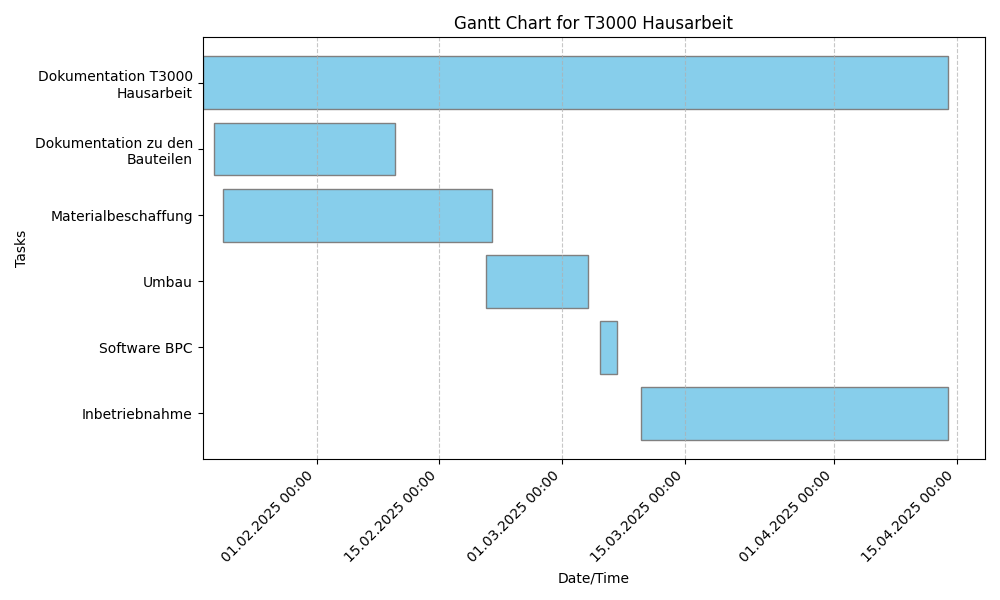
\includegraphics[width=1\linewidth]{images/Gantt_Chart.png}\\[1ex]
    \centering
    \caption{Gantt Chart T3000 Hausarbeit\label{ABBILDUNGEN}}
\end{figure}

\subsection{Planung und Vorbereitung}
Ein zentraler Bestandteil des Projekts war die Dokumentation der relevanten Bauteile. Dazu gehörten die Erfassung von Datenblättern,
 Verkabelungsinformationen sowie die Identifikation weiterer erforderlicher Komponenten. In Abstimmung mit Kollegen wurde geprüft, 
 welche Teile bereits vorhanden waren und welche noch beschafft werden mussten. Die fehlenden Bauteile wurden über das \ac{SAP}-System ausgebucht 
 und organisiert.

 \subsection{Umbau des Fahrzeugs}
 Der eigentliche Umbau des Fahrzeugs erfolgte in Zusammenarbeit mit Claus Vogt. Dabei wurden verschiedene
 mechanische und elektrische Anpassungen vorgenommen, um die neuen Bauteile zu integrieren. 
 Zu den durchgeführten Arbeiten gehörten:
 
 \begin{itemize}
    \item Modifikation der vorhandenen Hardwarekomponenten
    \item Installation der neuen Bauteile gemäß den technischen Spezifikationen
    \item  Anpassung der Verkabelung und Integration in das bestehende System
 \end{itemize}

 Besonderes Augenmerk lag auf der korrekten Pin-Belegung (Pinning) sowie der Montage der Bauteile im Fahrzeug, 
 die unter Anleitung und in Abstimmung mit Claus Vogt umgesetzt wurden.

 \subsection{Installation der BPC-Software}
Nach dem mechanischen Umbau wurde die \acs{BPC}-Software auf 
dem entsprechenden Controller installiert. Dies erforderte sowohl hardwareseitige Anpassungen
 als auch softwaretechnische Konfigurationen, die in Zusammenarbeit mit Daniel Sessler durchgeführt wurden. 
 Die korrekte Pin-Belegung (Pinning) wurde mithilfe relevanter Dokumentation überprüft und dokumentiert.

\subsection{Inbetriebnahme}
Nach der Installation und Validierung der neuen \acs{BPC}-Software wurde das Fahrzeug in Betrieb genommen und getestet. Dabei wurde überprüft, 
ob die Erwartungen an den neuen Fahrantrieb im \acs{PoC}-Fahrzeug erfüllt wurden.

Im Rahmen der Tests wurden alle relevanten Parameter kontrolliert und 
die Funktionalität der neu integrierten Komponenten sichergestellt. Dazu gehörten insbesondere:

\begin{itemize}
    \item Die neu eingebauten Keypads
    \item Das Rafi Gen2 Display
    \item Die Hill-Hold-Funktion
\end{itemize}

Durch die Inbetriebnahme konnte festgestellt werden, 
ob die geplanten Optimierungen erfolgreich umgesetzt wurden und das Fahrantriebskonzept 
die gewünschten Verbesserungen erzielt.
\end{spacing}

\section{Ergebnisse und Ausblick}
\begin{spacing}{1.5}  % Adjust line spacing
    \fontsize{14pt}{14pt}\selectfont  % Font size and line spacing
    Im Verlauf des Projekts konnten wertvolle Erkenntnisse gewonnen werden, die als Grundlage für zukünftige Weiterentwicklungen dienen. 
    Die Umsetzung des \acf{PoC}-Umbaus hat gezeigt, welche Optimierungen am Fahrantriebskonzept erfolgreich waren und welche
     Aspekte weiter verbessert werden können.

    Nach Abschluss dieser Phase wird das Projekt mit dem Umbau des Hydraulik-\acs{PoC} fortgesetzt. Anschließend 
    folgt die Beschaffung und Vorbereitung für den ersten Prototypenbau des Konzeptfahrzeugs. Die gewonnenen 
    Erfahrungen aus diesem \acs{PoC} fließen direkt in die nächste Entwicklungsstufe ein, um die Praxistauglichkeit und Effizienz 
    des neuen Fahrantriebskonzepts weiter zu optimieren.
    
    Langfristig dient dieses Projekt dazu, die Wettbewerbsfähigkeit der Kramer Telelader durch innovative 
    Technologien weiter zu steigern und die Effizienz sowie die Leistungsfähigkeit der Fahrzeuge nachhaltig
     zu verbessern.
\end{spacing}

\clearpage

%---------------------------------------------------------
% Bibliografie
%---------------------------------------------------------
\begingroup
\renewcommand{\bibfont}{\fontsize{13pt}{12pt}\selectfont}  
\sloppy
\nocite{*}
\printbibliography{}

\end{document}
